\chapter{Microservizio anagrafica}\label{cap:microservizio-anagrafica}

\section{Scopo del sistema}

Il sistema di anagrafica si occupa di gestire le informazioni anagrafiche dei sensori, delle aree e dei lampioni. Gestisce questi raggruppamenti e si occupa di renderli persistenti su database.

\section{Requisiti coperti dal sistema}

\subsection{RF\_03}
RF\_03:deve essere possibile aggiungere nuovi sensori a sistema.

Questo microservizio, copre il requisito peristendo i dati anagrafici del sensore.

\subsection{RF\_08}
RF\_08:l'utente deve poter inserire la locazione geografica del sensore nel sistema.

Questo microservizio, copre il requisito peristendo i dati di locazione del sensore.

\subsection{RF\_09}
RF\_09:l'utente deve poter inserire il raggio di azione del sensore.

Questo microservizio, copre il requisito peristendo i dati di raggio di azione del sensore.

\subsection{RF\_10}
RF\_10:l'utente deve poter essere in grado di visualizzare quali aree sono illuminate in un dato momento

Questo microservizio, copre parte del requisito fornendo l'informazione di quali lampioni si trovano in una determinata area.



\section{Descrizione del sistema}

Il sistema principalmente fornisce le informazioni stoccate su base dati tramite un'interfaccia rest.
Questo è poi in grado di fornire i dati in forma aggregata, come ad esempio il numero di lampioni per area, o il numero di sensori per lampioni.

Per queste informazioni ha inoltre il compito e la responsabilità di tenere aggiornati i dati nel database, organizzando i dati in modo da poterli fornire in modo efficiente.

\section{Architettura del sistema}

L'architettura base del sistema è sviluppata in ottica KISS.

Il sistema è composto da un'interfaccia rest che espone i dati e da un insieme di classi che si occupano di gestire i dati nel database.

Il servizio nasce molto semplice e per questo motivo non è stato ritenuto necessario l'utilizzo di un'architettura più complessa e strutturata.

Ognuna delle classi rispetta però SOLID e soprattutto il principio della singola responsabilità.

\begin{figure}[ht]
    \centering
    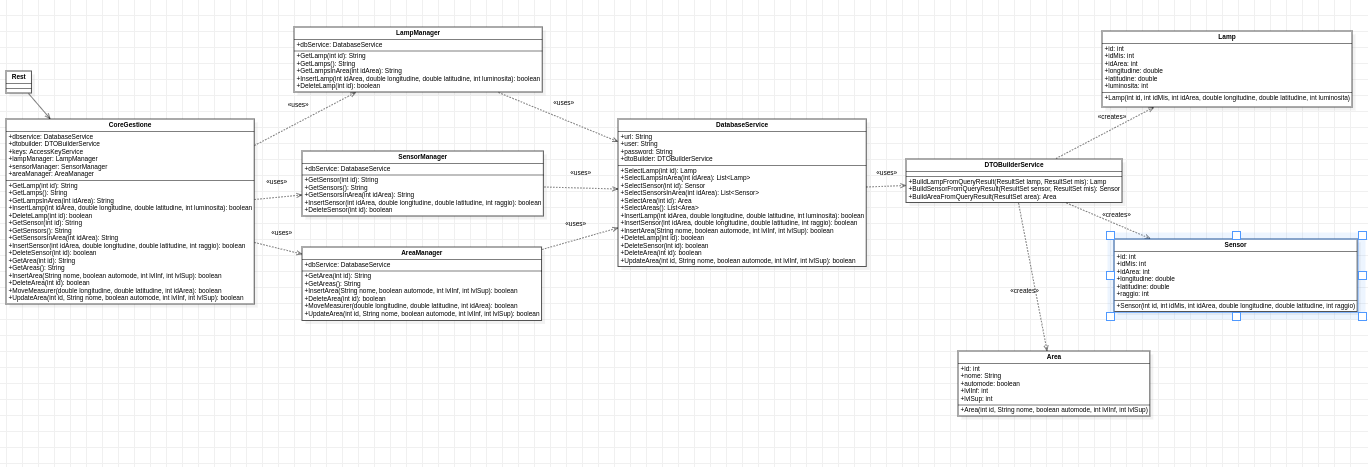
\includegraphics[width=\textwidth]{img/anagrafe_generale.png}
    \caption{Vista generale del sistema di anagrafe, si consiglia visione nel dettaglio delle immagini \ref{fig:services_anagrafe}, \ref{fig:managers_anagrafe} e \ref{fig:core_anagrafe}}
    \label{fig:general_anagrafe}
\end{figure}

\section{Servizi}

I servizi sono in generale le interfaccie ad alto livello delle funzionalità del sistema. Sono composti da classi che si occupano di gestire le richieste e di fornire i dati richiesti.
Questi si possono essere visionati nell'immagine \ref{fig:services_anagrafe}.

\begin{figure}[ht]
    \centering
    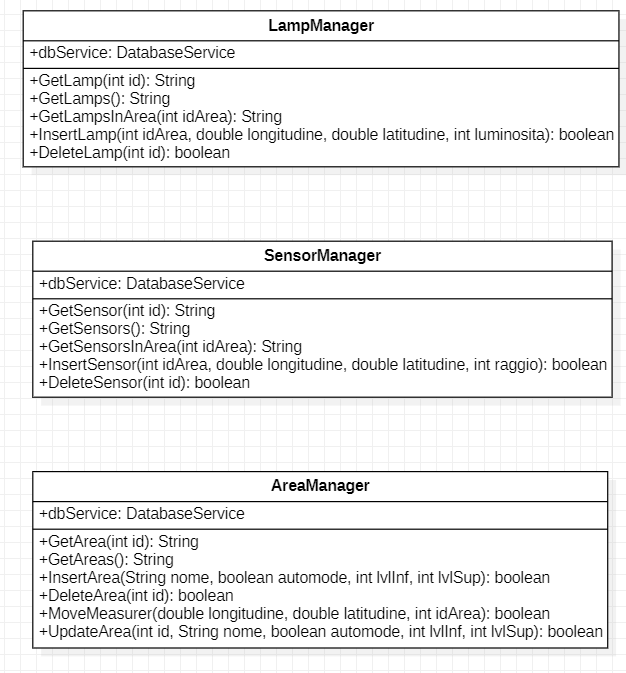
\includegraphics[width=\textwidth]{img/services_anagrafe.png}
    \caption{Diagramma delle classi del modello all'interno del sistema di anagrafe}
    \label{fig:services_anagrafe}
\end{figure}

\subsection{DatabaseService}

DatabaseService si occupa di effettuare tutte le operazioni di connessione e interazione con il database. 

Sono presenti operazioni di Select, Delete, Insert e Update. In futuro può essere espandibile in base al tipo di operazione che si desidera fare.

\subsection{DTOBuilderService}
DTOBuilderService si occupa di creare i diversi DTO dell'applicazione, in questo caso Area, Lampione e Sensore, che verranno utilizzate all'interno dell'applicazione per muovere i dati tra le varie parti del sistema.

\subsection{AccessKeysService}
L'AccessKeysService si occupa di verificare che la chiave di accesso dell'utente non sia scaduta. Se la chiave è valida l'utente può utilizzare le varie funzionalità offerte dal microservizio.

\section{Interfaccia REST}

L'interfaccia rest viene esposta all'esterno e permette di effettuare le operazioni discusse nelle sotto-sezioni successive.

Questa interfaccia comunica al resto del sistema tramite il componente \textit{CORE} definito nella sezione \ref{sec:core}.

\begin{itemize}
    \item GET /getLamp/id
    \item GET /getLampsInArea/idArea
    \item PUT /addLamp
    \item PUT /deleteLamp/id
    \item GET /getSensor/id
    \item GET /getSensorsInArea/idArea
    \item PUT /addSensor
    \item PUT /deleteSensor/id
    \item PUT /moveMeasurer/idMeasurer
    \item GET /getArea/id
    \item GET /getAreaList
    \item PUT /addArea
    \item PUT /updateArea/id
    \item PUT /deleteArea/id
\end{itemize}

\subsection{ GET /getLamp/id}

GetLamp permette di ottenere tutti i dati relativi a un lampione. L'utente deve fornire l'id del lampione in questione.

Il sistema risponderà con un JSON contenente tutti i dati relativi al lampione richiesto.

\subsection{ GET /getLampsInArea/idArea}

GetLampsInArea permette di ottenere i dati relativi a tutti i lampioni in un'area. L'utente deve fornire l'id dell'area della quale si desidera visualizzare i lampioni.

Il sistema risponderà con un JSON contenente tutti i dati relativi ai lampioni presenti in quell'area.

\subsection{ PUT /addLamp}

AddLamp permette di inserire nel database un nuovo lampione. All'utente è richiesto di fornire i dati relativi al lampione da inserire in un JSON che viene inviato al sistema.

Il sistema risponderà con un boolean ad indicare se l'operazione è andata a buon fine o meno.

\subsection{ PUT /deleteLamp/id}

DeleteLamp permette di eliminare dal database un lampione. L'utente deve fornire al sistema l'id del lampione da eliminare.

Il sistema procede poi a tentare di eliminare il lampione, rimuovendo prima il riferimento al misuratore, e ritorna un boolean positivo in caso di successo, negativo in caso di fallimento.

\subsection{ GET /getSensor/id}

GetSensor permette di ottenere tutti i dati relativi a un sensore. L'utente deve fornire l'id del sensore in questione.

Il sistema risponderà con un JSON contenente tutti i dati relativi al sensore richiesto.

\subsection{ GET /getSensorsInArea/idArea}

GetSensorsInArea permette di ottenere i dati relativi a tutti i sensorioni in un'area. L'utente deve fornire l'id dell'area della quale si desidera visualizzare i sensorioni.

Il sistema risponderà con un JSON contenente tutti i dati relativi ai sensorioni presenti in quell'area.

\subsection{ PUT /addSensor}

AddSensor permette di inserire nel database un nuovo sensore. All'utente è richiesto di fornire i dati relativi al sensore da inserire in un JSON che viene inviato al sistema.

Il sistema risponderà con un boolean ad indicare se l'operazione è andata a buon fine o meno.

\subsection{ PUT /deleteSensor/id}

DeleteSensor permette di eliminare dal database un sensore. L'utente deve fornire al sistema l'id del sensore da eliminare.

Il sistema procede poi a tentare di eliminare il sensore, rimuovendo prima il riferimento al misuratore, e ritorna un boolean positivo in caso di successo, negativo in caso di fallimento.

\subsection { PUT /moveMeasurer/id}

MoveMeasurer permette di spostare un misuratore (che può essere un lampione o un sensore) da un'area a un'altra. L'utente deve fornire l'id del misuratore da spostare e un JSON contenente le nuove coordinate e l'area dove va inserito.

Il sistema ritorna infine un boolean positivo in caso di successo, negativo in caso di fallimento.

\section{Managers}

\begin{figure}[ht]
    \centering
    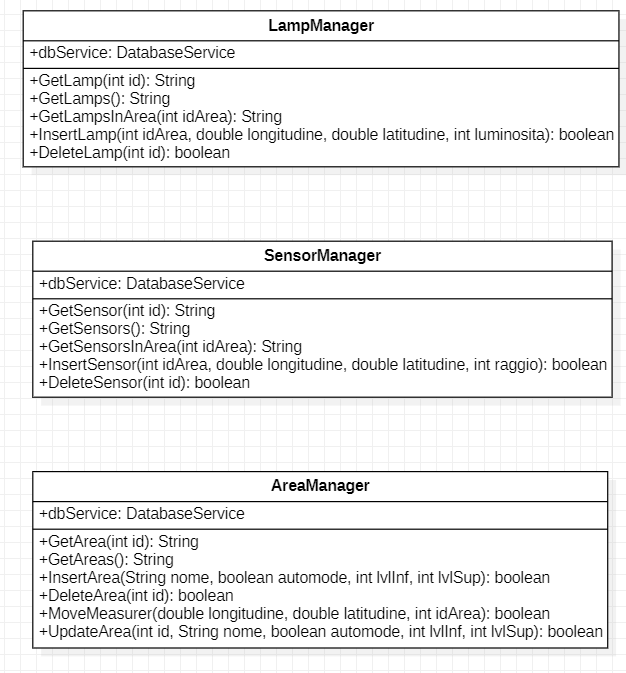
\includegraphics[width=0.5\textwidth]{img/managers_anagrafe.png}
    \caption{Diagramma delle classi relative ai servizi del sistema di anagrafe}
    \label{fig:managers_anagrafe}
\end{figure}

Si occupano di fare da tramite tra il servizio che colloquia fisicamente con il DB e il controller che si occupa di gestire le richieste REST.
Si possono vedere i metodi dei servizi nel diagramma delle classi \ref{fig:managers_anagrafe}.

\begin{itemize}
    \item \textbf{LampManager}: si occupa della gestione (ottenimento, inserimento, modifica o cancellazione) dei dati relativi ai lampioni nel database.
    \item \textbf{SensorManager:} si occupa della gestione (ottenimento, inserimento, modifica o cancellazione) dei dati relativi ai sensori nel database. 
    \item \textbf{AreaManager:} si occupa della gestione (ottenimento, inserimento, modifica o cancellazione) dei dati relativi alle aree nel database.
\end{itemize}

\paragraph{LampManager}

Ha la responsabilità di gestire l'inserimento e la rimozione di un lampione dal database, oltre che di ottenere i dati relativi a un lampione o a tutti i lampioni in un'area.

\paragraph{SensorManager}

Ha la responsabilità di gestire l'inserimento e la rimozione di un sensore dal database, oltre che di ottenere i dati relativi a un sensore o a tutti i sensori in un'area.

\paragraph{AreaManager}
Ha la responsabilità di gestire l'inserimento e la rimozione di un'area dal database, oltre che di ottenere i dati relativi a un'area o a tutte le aree.

\section{Core}\label{sec:core} L'interfaccia accentra tutte le funzionalità base del sistema rendendo semplice l'implementazione di nuove interfaccie esterne all'utente.

Tutti i suoi metodi sono statici e permettono di ottenere i dati dal database in modo semplice e veloce.

I metodi che questa componente offre sono visibili nel diagramma delle classi \ref{fig:core_anagrafe}.

\begin{figure}[ht]
    \centering
    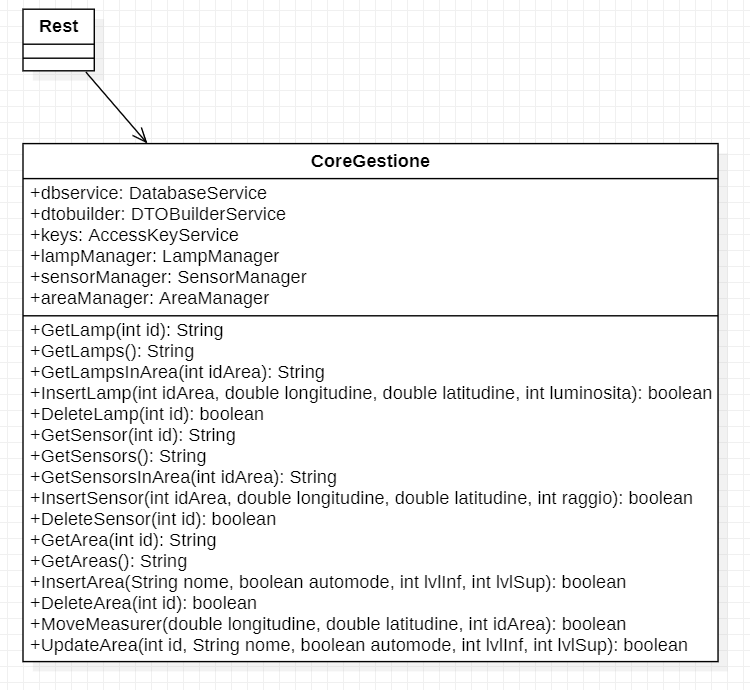
\includegraphics[width=0.5\textwidth]{img/core_anagrafe.png}
    \caption{Diagramma delle classi relative al core del sistema di anagrafe}
    \label{fig:core_anagrafe}
\end{figure}
